\chapter{Implementación}

\section{Algoritmos de clasificación}

Se implementaron 2 algoritmos de clasificacion: Busqueda lineal y Busqueda en árbol unibit.

El software utilizado para realizar las pruebas consistió en 2 proyectos por separado. Uno para cada tipo de búsqueda en la tabla.

El mismo fue desarrollado en lenguaje c++, por presentar éste ciertas facilidades para las implementaciones llevadas a cabo. Puntualmente se sacó ventaja de un STL container (list) para implementar la búsqueda lineal. La característica utilizada en este caso fue el ordenamiento de la lista con sólo una llamada a función.

Para efectuar el intercambio de datos con el hardware se hizo uso de las macros IOWR e IORD, las cuales escriben y leen respectivamente los datos hacia/desde un componente conectado al bus Avalon MM. La razón de haber usado dichas macros yace en el hecho de que las mismas no son puestas en caché. Esta característica se torna indispensable en este diseño, ya que en el mismo no se puede leer un dato sin saber si está verdaderamente disponible en el bus.


\subsection {Búsqueda lineal}

Se implementaron 2 clases. 

\begin{itemize}
	\item \textit{iproute.h}: define el contenido de cada nodo de la lista (entrada en la tabla de ruteo).
	\item \textit{iplookup.h} -  contiene la lista que constituye la tabla de ruteo en sí, así como también las funciones de inserción y búsqueda. También contiene la función que crea una tabla de ruteo de 100 entradas.
\end{itemize}

Los nodos de la lista contienen 3 campos:

\begin{itemize}
	\item Dirección de red (entero de 32 bit sin signo)
	\item Máscara de red (entero de 32 bit sin signo)
	\item Identificador de decisión (entero de 32 bit con signo)
\end{itemize}

Como se le dió prioridad a los prefijos de red más largos, se debió sobrecargar el operador de comparación ( > ) para que la función sort pudiese ordenar en base a la longitud de máscara. De esa manera, los nodos que contenían valores de máscara más grandes quedaban en las primeras posiciones de la lista.

La función de inserción toma como entrada una dirección, una máscara y un identificador de decisión. Luego instancia una entrada con dichos elementos y la inserta en la lista.

Cuando la función encargada del lookup recibe una dirección IP de destino, realiza los siguientes pasos:

\begin{itemize}
	\item Coloca un iterador al comienzo de la lista.
	\item Realiza un AND con el valor de máscara del nodo que está siendo apuntado. Si el resultado de la operación es igual al valor de dirección de red de dicho nodo, entonces se retorna con el valor identificador de decisión. En otro caso, continúa la busqueda en el siguiente nodo.
\end{itemize}

\subsection {Busqueda en Arbol unibit}

Se implementaron 2 clases. 

\begin{itemize}
	\item \textit{trienode.h}: define las características de cada nodo del árbol.
	\item \textit{trie.h}: contiene el árbol unibit, como así tambien las funciones de búsqueda e inserción de nodos. También contiene una función para la creación de la tabla de ruteo de 100 valores.
\end{itemize}


En este contexto, pueden existir 2 tipos de nodo:

\begin{itemize}
	\item Común: no está asociado a una decisión.
	\item Decisión: contiene un valor que identifica a la decisión a tomar. 
\end{itemize}

Cada nodo cuenta con los siguientes campos:
\begin{itemize}
	\item gw: es un identificador de la decisión a tomar. En los nodos no asociados a una decision (nodos comunes), tiene el valor estipulado en la macro NONE.
    \item zero / one: Son punteros a nodo, asociados a los bits 0/1 del prefijo que se esté leyendo.

\end{itemize}

La función de inserción toma como entrada una dirección y una máscara de red, así como también un valor de decisión asociado a la entrada en tabla. Lleva a cabo los siguientes pasos:
\begin{itemize}
	\item Partiendo con un puntero de recorrido desde el nodo raíz, el procedimiento se encuentra contenido en un bucle controlado por la longitud de la máscara de red. Es decir, en cada iteración se hace un testeo de bit de dicha máscara. 
	\item Si éste es igual a uno, la iteración se lleva a cabo.
	\item En ella, se hace un testeo de bit pero de la dirección de red.
	\item Si el mismo es igual a cero, se desplaza el puntero de recorrido hacia el nodo apuntado por \textit{zero}.
	\item En caso de no existir dicho nodo, se lo crea y recién ahí se desplaza el puntero de recorrido.
	\item Un procedimiento análogo se lleva a cabo en caso de que el testeo de bit sea igual a uno.
	\item Una vez finalizado el bucle, se escribe el valor de decisión en el nodo que esté siendo apuntado por el puntero de recorrido.
\end{itemize}


El algoritmo de búsqueda toma como entrada la dirección IP de destino del paquete a clasificar. Luego de ello realiza las siguientes acciones:
\begin{itemize}
	\item Va haciendo un testeo bit a bit de dicha dirección, partiendo con un puntero de recorrido desde el nodo raíz.
	\item Si el bit de la dirección es 0 y el puntero zero está apuntando hacia algún nodo, el puntero de recorrido se mueve al nodo apuntado por el puntero zero.
	\item En caso contrario, se mueve al nodo apuntado por el puntero one (En caso de que exista alguno).
\end{itemize}

Esto se repite nodo a nodo, hasta que ocurre alguna de las siguientes situaciones:

\begin{itemize}
    	\item El puntero de recorrido queda varado en un nodo decision, con lo cual se retorna el valor de gw.
    	\item El puntero de recorrido queda varado en un nodo común. 
\end{itemize}


Contemplando esta última posibilidad, el algoritmo hace que en cada nodo se chequee si se trata de un nodo decisión. En dicho caso, se almacena el campo gw en una variable y se continua el recorrido. Si se da un caso en el cual el nodo de recorrido queda apuntando a un nodo comun y luego de testear un bit se determina que el mismo no tiene un nodo asociado (es decir, que alguno de los punteros zero / one esté en NULL) la función retorna la variable anteriormente mencionada. 

Cabe mencionar también que la ruta por defecto se inserta en el nodo raíz del arbol.

\begin{figure}[H]
  \centering
	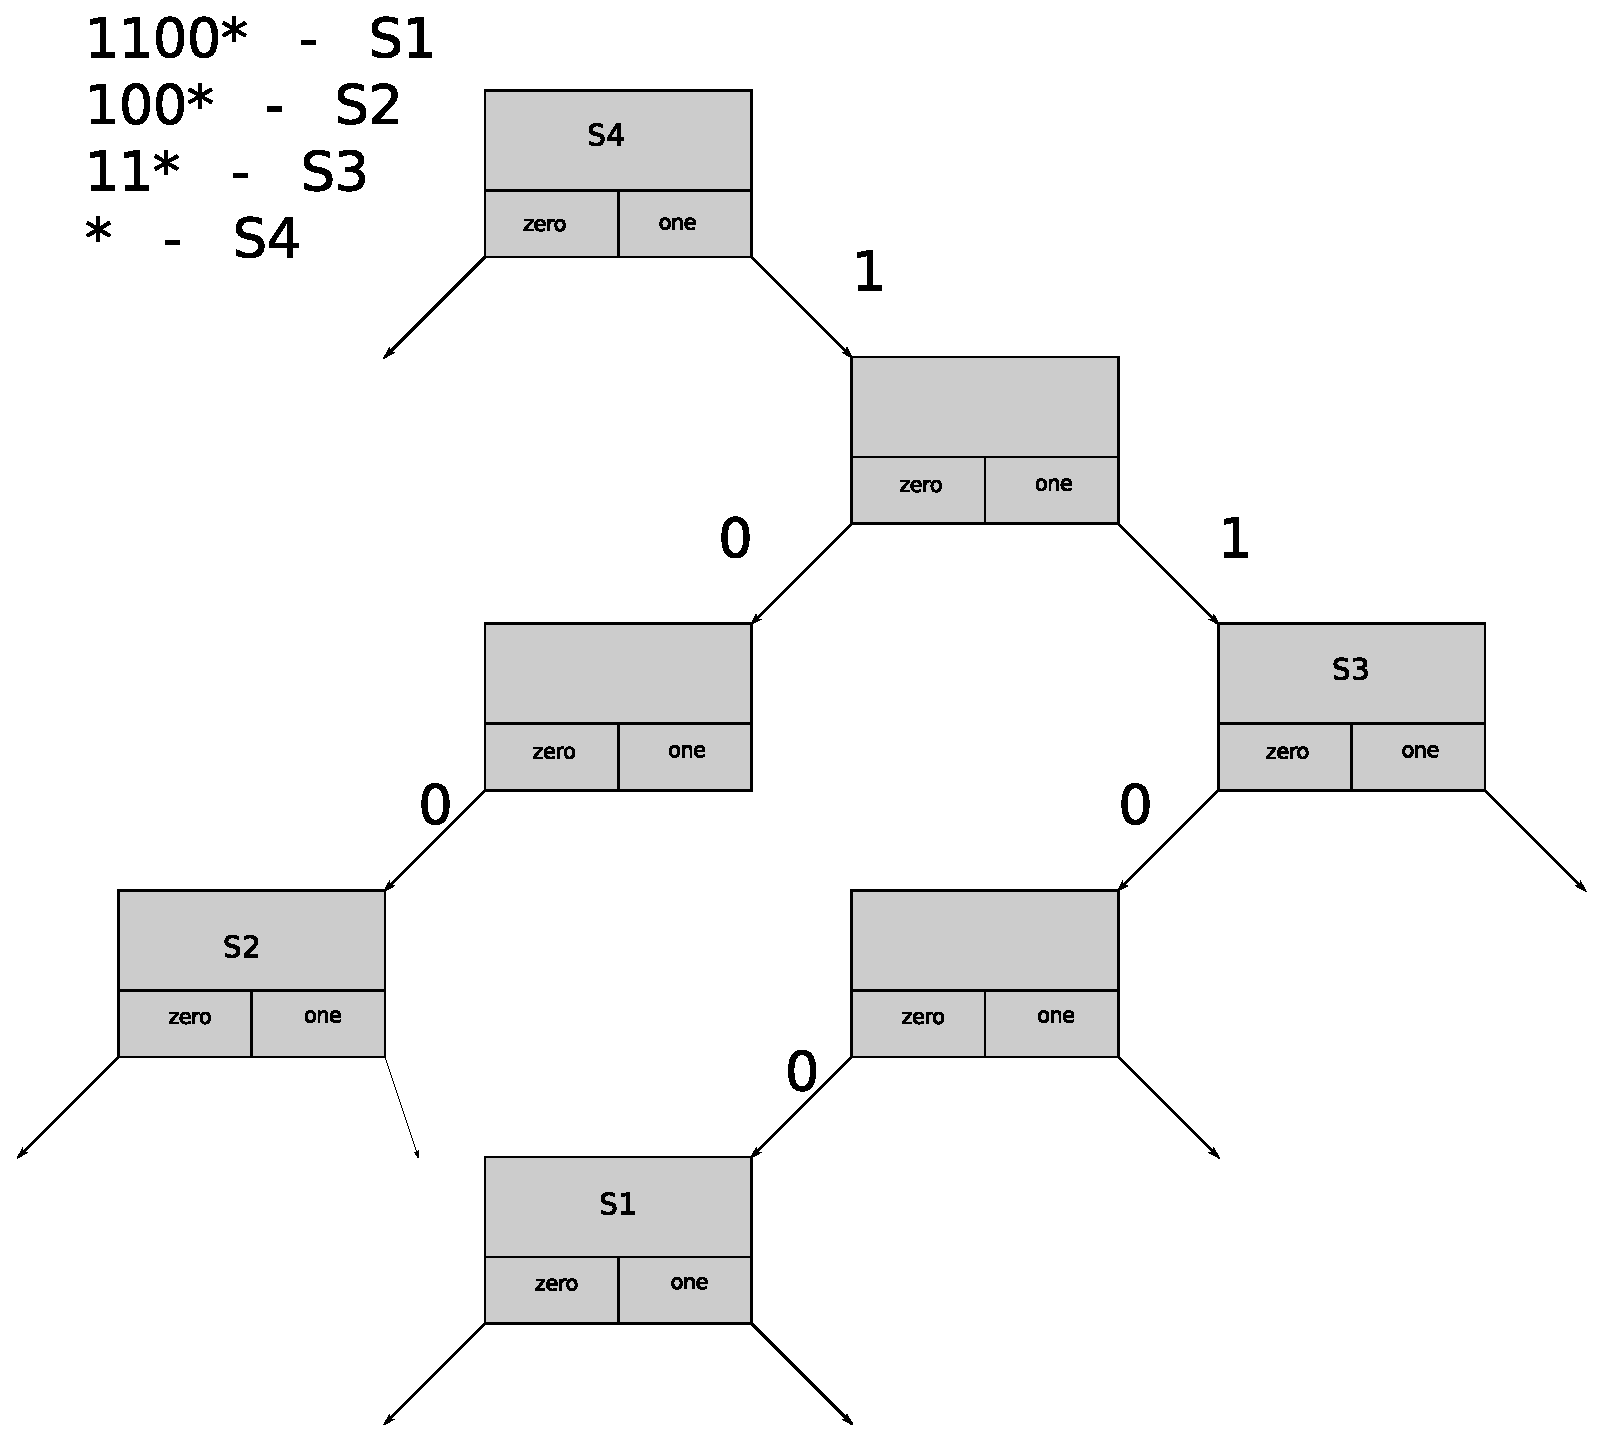
\includegraphics[scale=0.50]{4-implementacion/graf/lluinsert09.eps}
  \caption{Ejemplo de inserción de prefijos en árbol unibit}
  \label{fig:lluinsert}
\end{figure}

En la figura ~\ref{fig:lluinsert} se encuentra ejemplificada la inserción de 3 prefijos más la ruta por defecto. 

Comenzando por el nodo raíz, se inserta el prefijo 1100*. Para ello es necesaria la creación de 4 nodos hijos, uno por cada bit del prefijo. 

A continuación es insertado el prefijo 100*. Para el primer bit ya se encuentra creado el nodo, por lo cual se crean los 2 restantes necesarios.

Luego se inserta el prefijo 11*. Como anteriormente se había insertado el 1100* los nodos necesarios ya existen, por lo cual la inserción es trivial.

Por último en el nodo raíz se inserta la ruta por defecto (S4 en este ejemplo).

Tomando como ejemplo alguna dirección IP que comienze con 1100, puede verse que la búsqueda tomará el camino \textit{Raíz - one - one - zero - zero} y culminará en el nodo cuyo identificador de decisión es S1. 

Vale la pena considerar qué sucede si la dirección IP comienza con 1101. En este caso el camino que seguirá la búsqueda es \textit{Raiz - one - one - zero} y el puntero de recorrido quedará varado allí, ya que no existe en dicho punto un nodo asociado al puntero one. Vale recordar que en cada iteración, el algoritmo de búsqueda chequea si el nodo apuntado por el puntero de recorrido es decisión. Para este caso puede verse que en la segunda iteración (cuando se ha recorrido \textit{Raíz - one - one}) el algoritmo se encuentra parado en un nodo decisión y por lo tanto almacena el valor contenido en dicho nodo y procede a continuar. Cuando se encuentre varado en el próximo, lo que hará es retornar con el valor mencionado anteriormente. 

\subsection {Cache}

Se implementó una cache directa. La misma consta de una tabla hash de 16 entradas, aunque este tamaño puede ser modificado mediante la macro CACHE\_SIZE. Las colisiones se resuelven por reemplazo directo. La misma fue testeada con ambos algoritmos mencionados anteriormente. Para ello, se agregó una lógica adicional que consistió en:

\begin{itemize}
	\item Al tomar una direccion IP, chequear primero si el valor de decisión se encuentra en caché.
	\item Si está, retornar dicho valor.
	\item En otro caso, efectuar el lookup y almacenar el valor de decisión en caché. Para dicho almacenamiento, se efectúa un hash en la dirección IP, que consiste en calcular el resto de la división entre dicha dirección y el valor de CACHE\_SIZE. El resultado es utilizado como índice para el almacenamiento en la tabla.
\end{itemize}

Para evitar el overhead introducido por el uso de clases, se optó por una implementación basada en una estructura, a la cual se denominó \textit{HashEntry}. La misma cuenta con los siguientes campos:

\begin{itemize}
	\item address: Dirección IP almacenada.
	\item gw: Identificador de decisión.
	\item empty: Indica si la entrada de tabla está vacía.
\end{itemize}

\section{ISR}

Como se mencionó anteriormente, el módulo Uplink envía interrupciones al procesador. A fin de poder procesarlas en el software se implementó una ISR (Interrupt Service Routine) que hace uso de 3 elementos principales:

\begin{itemize}
	\item \textit{store\_array}: Es un buffer en el cual se van almacenando las palabras enviadas por el módulo Uplink.
	\item \textit{i}: Es un subíndice que sirve para moverse dentro del buffer anteriormente mencionado.
	\item \textit{flag}: Es un indicador que se incrementa cada vez que se produce una interrupción.
\end{itemize}

\textit{store\_array} está implementado como una matriz de enteros, y tiene 3 columnas. De esta manera, cada fila cuenta con con 96 bits de los cuales se utilizan 72 de ellos para almacenar las palabras enviadas por Uplink.

Cada vez que el procesador recibe una interrupción, lleva a cabo la lectura del valor recibido y la almacena en \textit{store\_array}, en el lugar indicado por \textit{i}. Luego el subíndice se incrementa, al igual que \textit{flag}.

En la función principal (main) existe una variable llamada \textit{flag2}. A ésta se le asigna el valor de \textit{flag}. Al producirse una interrupción, el valor de \textit{flag} se modifica y por lo tanto la condición de igualdad entre \textit{flag} y \textit{flag2} ya no se cumple. En ese momento se utilizan los valores almacenados en \textit{store\_array} para llevar a cabo el algoritmo de clasificación. Dichos valores a utilizar dependerán de la versión de Uplink que se esté utilizando:

\begin{itemize}
	\item Para la versión que envía quince palabras de 32 bits, es necesario esperar a la quinta palabra de 96 bits en \textit{store\_array} para poder localizar la dirección IP de destino, necesaria para realizar la clasificación. En la figura ~\ref{fig:ip15pal} se muestra cómo está localizada dicha dirección. 
	\item Para la versión que envía sólo una palabra de 32 bits, el procedimiento es trivial ya que esa misma palabra es la dirección IP de destino.
\end{itemize}


Una vez llevado a cabo el procedimiento de clasificación, \textit{flag2} es puesto de nuevo al valor de \textit{flag }y el proceso se repite.


\begin{figure}[H]
  \centering
	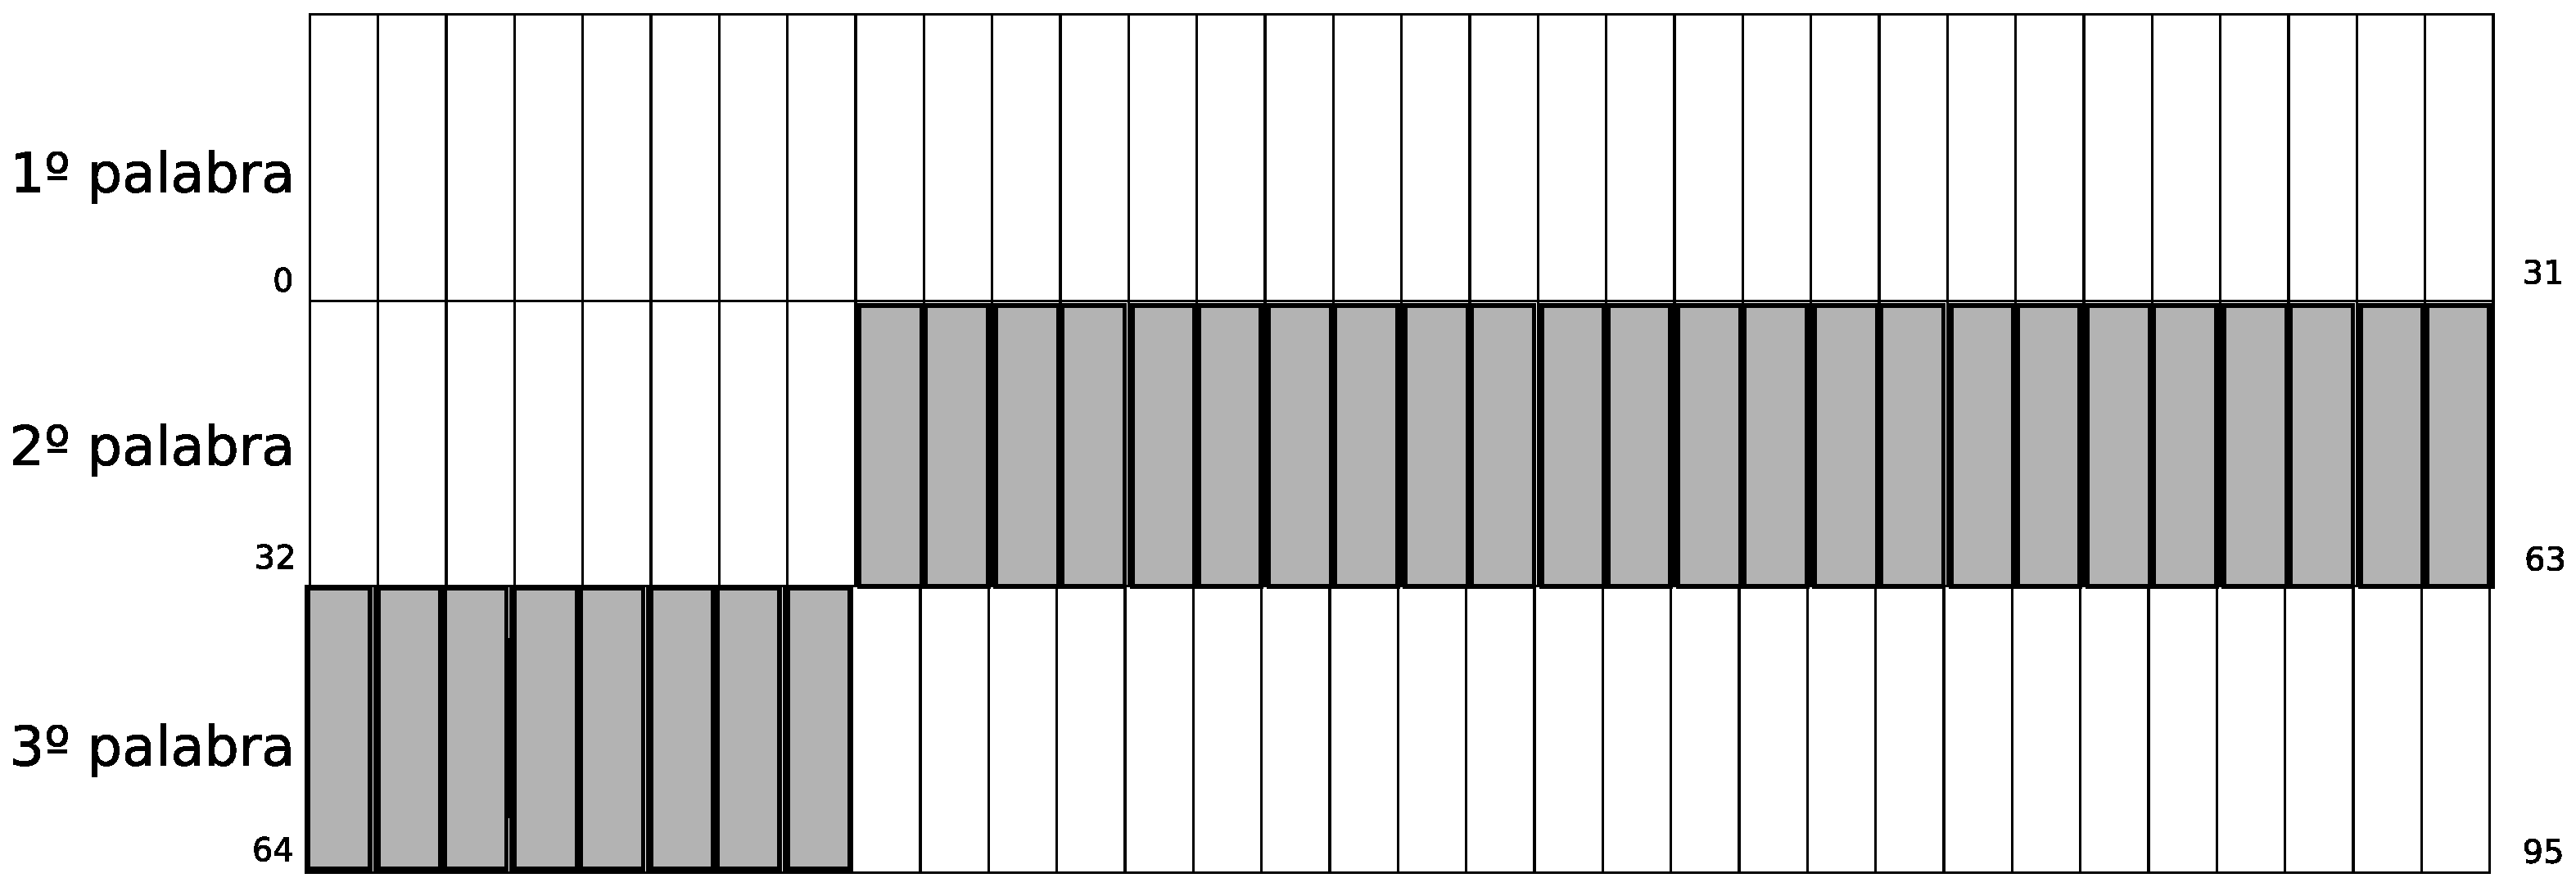
\includegraphics[scale=0.10]{4-implementacion/graf/ip15pal.eps}
  \caption{Ubicación de la dirección IP dentro de una palabra de 96 bits en store\_array, para la versión de Uplink que envía 15 palabras de 32 bits}
  \label{fig:ip15pal}
\end{figure}


\section{Hardware}

El hardware utilizado fue la placa de desarrollo DE2, cuyas características principales son:

\begin{itemize}
	\item FPGA: Cyclone II EP2C35F672C6
	\item USB Blaster integrado, para configuración de FPGA
	\item Memoria: 8 MB SDRAM, 512 KB SRAM, 4 MB Flash
	\item Clock de 50 MHz
\end{itemize}

Para una descripción más detallada, referirse al Apéndice A.

A su vez, la FPGA incluida en esta placa cuenta con estas características:

\begin{itemize}
	\item Elementos lógicos: 33216
	\item Bit totales de RAM: 483840
	\item Multiplicadores embebidos: 35
	\item PLLs: 4
	\item Cantidad máxima de pines definidos por el usuario: 475
\end{itemize}


\section{Microprocesador NIOS II}
El Nios II es un procesador RISC de 32 bits de propósito general que cuenta con las siguientes especificaciones:
\begin{itemize}
	\item Set de instrucciones, bus de datos y espacio de direcciones de 32 bits.
	\item 32 registros de propósito general.
	\item Soporte de hasta 32 interrupciones.
	\item Controlador de interrupciones externas para soportar una mayor cantidad de interrupciones.
	\item Multiplicación y división en una sola instrucción de 32 x 32 produciendo un resultado de 32-bits.
	\item Instrucciones dedicadas para multiplicaciones con resultados de 64 y 128 bits.
	\item Acceso a una variedad de periféricos e interfases a memorias  y periféricos fuera del chip.
	\item Modulo de depurado asistido por hardware.
	\item Unidad de manejo de memoria (MMU) opcional para soportar sistemas operativos mas complejos.
	\item Unidad de protección de memoria (MPU) opcional.
	\item Entorno de desarrollo de software basado en GNU C/C++ integrado a Eclipse.
	\item Integración con SignalTap® II, el analizador de lógica embebida de Altera permitiendo el análisis de tiempo real de todas las señales presentes en la FPGA.
	\item Set de instrucciones compatible entre todos las versiones del procesador Nios II.
\end{itemize}

Para poder ser implementado en una mayor variedad de dispositivos el Nios II ofrece 3 configuraciones diferentes:  Nios II/f (fast), Nios II/s (standard), and Nios II/e (economy).

\subsubsection{Nios II/e}
El Core Nios II/e esta diseñado para utilizar la menor cantidad de espacio posible. Esto esto funciona especialmente para FPGA de bajo costo. Tiene las siguientes características:
\begin{itemize}
	\item Espacio de direcciones de hasta 2GB
	\item Gratuito, no requiere licencia 
\end{itemize}

\subsubsection{Nios II/s}
El Nios II/s esta diseñado para mantener un balance entre rendimiento y costo. Entre sus características principales están:

\begin{itemize}
	\item Cache de instrucciones
	\item Espacio de direcciones de hasta 2GB
	\item Pipeline de 5 etapas
	\item Predictor de saltos estático
	\item Multiplicador y divisor por hardware. 
\end{itemize}

\subsubsection{Nios II/f}
El core Nios II/f esta diseñado para ofrecer la mayor performance a las expensas de un mayor tamaño, medido en unidades lógicas, este core tiene las siguientes características:

\begin{itemize}
	\item Cache de instrucciones y de datos separadas
	\item MMU y MPU opcionales
	\item Espacio de direcciones de hasta 2GB
	\item Pipeline de 6 etapas
	\item Multiplicador por hardware en un ciclo
	\item Divisor por hardware opcional
	\item Predictor de saltos dinámico
\end{itemize}

En vista de que este último ofrece la mayor performance y el hardware utilizado es capaz de soportarlo, se optó por el mismo para ser instanciado en el sistema.


\subsection{Verificación y síntesis}

La figura ~\ref{fig:fpga} muestra el porcentaje de uso de los recursos de la FPGA utilizada.

\begin{figure}[H]
  \centering
	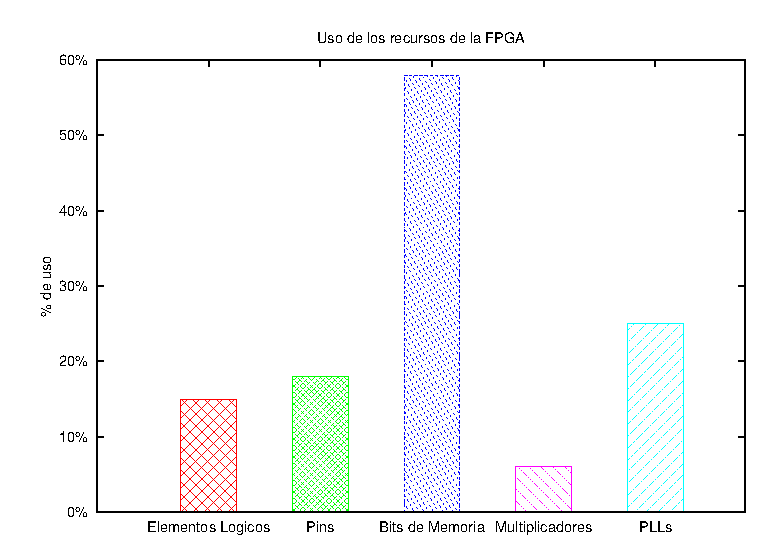
\includegraphics[scale=0.70]{4-implementacion/graf/fpga.eps}
  \caption{Uso de los recursos de la FPGA}
  \label{fig:fpga}
\end{figure}

%\section{Distribucion Lineal}
